\documentclass[output=paper,colorlinks,citecolor=brown,
% hidelinks,
% showindex
]{langscibook}
\author{Rachel Weiher\affiliation{University of California, Berkeley}}
\title{Factors of lexical stability in (inter)action across Romance}
\abstract{In the historical development of the Romance languages, preservation of Latin lexical forms in modern Romance has been posited to be resultant of a series of linguistic factors, among which are material stability (i.e. persistence of use/relevance to the community or culture) and emotivity (i.e. degree of emotive value) \citep[578--580]{stefenelli_lexical_2011}. Following Stefenelli’s proposal, as a quantitative assessment of the relative effects of these linguistic factors on Romance lexical stability, the present study examines the preservation and innovation of a stratified random sampling of basic vocabulary in Latin \citep{swadesh_towards_1955} coded for material stability and emotivity across Italian, Portuguese, Spanish, Catalan, French and Romanian. Results of regression modeling in R \citep{r_core_team_r_2019} indicate that material stability favors preservation, yet a significant interaction between material stability and emotivity illustrates a nullifying effect of emotivity when the two factors act in tandem. Thus, results lend evidence in support of the more impressionistic claims made in \cite{stefenelli_lexical_2011} and underscore the importance of combining qualitative and quantitative methodologies in the advancement of historical linguistic theory.}

\IfFileExists{../localcommands.tex}{%hack to check whether this is being compiled as part of a collection or standalone
   % add all extra packages you need to load to this file

\usepackage{tabularx,multicol,multirow}
\usepackage{url}
\urlstyle{same}

\usepackage{listings}
\lstset{basicstyle=\ttfamily,tabsize=2,breaklines=true}

\usepackage{langsci-basic}
\usepackage{langsci-optional}
\usepackage{langsci-lgr}
\usepackage{langsci-gb4e}
%    \let\eachwordone=\it % Ch 14, 18

\usepackage{jambox}
\usepackage{subfigure}
\usepackage{tablefootnote}
\usepackage[nameinlink, noabbrev]{cleveref}
\crefname{enumi}{example}{examples}

\usepackage{bbding}
%\usepackage{linguex}
\usepackage{stmaryrd}

\usepackage{tipa}
\let\ipa\textipa
\usepackage{vowel}
\newcommand{\BlankCell}{}
\usepackage{ot-tableau}

\usepackage{forest}
\useforestlibrary{linguistics}
\usepackage[noeepic]{qtree}
\usepackage{pstricks, pst-xkey, pst-jtree}
\usepackage{tikz-qtree}
\usepackage{tikz-qtree-compat}
\usepackage{tree-dvips}

\usepackage{lastpage}
\usepackage{hyperref}
\usepackage{xltxtra}

\usepackage{ragged2e}
%\usepackage{subcaption}
\usepackage{floatrow}
\usepackage{float}

\usepackage[normalem]{ulem} % Pour les textes barrés
\usepackage{ifthen} 

\usepackage{todonotes}

   \newcommand*{\orcid}{}

\makeatletter
\let\theauthor\@author
\makeatother

\papernote{\scriptsize\normalfont
    \theauthor.
    \titleTemp. 
    To appear in: 
    Chad Howe and Pilar Chamorro and Timothy Gupton and Margaret Renwick.
    Theory, Data, and Practice: Selected papers from the 49th Linguistic Symposium on Romance Language
    Berlin: Language Science Press. [preliminary page numbering]
}

% Workaround for subscripts with capital letters
\newcommand{\capsub}[1]{\ensuremath{_\text{#1}}}

% Chapter 10: Table-like presentation within example environment
% classical latin > {*}late latin > old french  earlier > later   gloss
\newcommand{\montanoboxi}[7]{\parbox{2cm}{#1} > {#2}\parbox{2cm}{#3} > \parbox{1.5cm}{\textit{#4}} \parbox{1.2cm}{#5}\ > \parbox{1.2cm}{#6} \parbox{1.5cm}{#7}}
% {*}latin > earlier OF [ipa] > early OF   gloss
\newcommand{\montanoboxii}[6]{{#1}\parbox{1.9cm}{\textit{#2}} > \parbox{1.3cm}{\textit{#3}} \parbox{2cm}{#4} \parbox{2cm}{#5} \parbox{1.9cm}{#6}}

% Chapter 5
\newcommand{\redc}[1]{\textcolor{red}{#1}}
\newcommand{\bluec}[1]{\textcolor{blue}{#1}}
\newcommand{\ajout}[1]{\textcolor{blue}{#1}}
\newcommand{\ajoutplus}[1]{\textcolor{cyan}{#1}}

\newcommand{\hachure}[9]{
% Parametres :
% Coordonnees bas gauche (2 parametres) : (#1,#2)
% Coordonnees haut droit (2 parametres) : (#3,#4)
% Orientation : #5
%   1 : diagonale de pente 1
%  -1 : diagonale de pente -1
%   0 : horizontal
%   2 : vertical
% Nombre de pas horizontaux : #6
% Epaisseur du trait : #7
% Couleur : #8 (ex. green)
% Atténuation couleur : #9 (ex. 30)
\pgfmathsetmacro{\N}{#6-1}
\pgfmathsetmacro{\A}{#1}
\pgfmathsetmacro{\B}{#2}
\pgfmathsetmacro{\C}{#3}
\pgfmathsetmacro{\D}{#4}
\pgfmathsetmacro{\I}{(#3-#1)/#6}
\pgfmathsetmacro{\J}{(#4-#2)/#6}
\ifthenelse{\equal{#5}{1}}{
  \foreach \n in {0,...,\N}
    \foreach \m in {0,...,\N}
      {
        \pgfmathsetmacro{\X}{\A + ((0 + \n) * \I)}
        \pgfmathsetmacro{\Y}{\B + ((0 + \m) * \J)}
        \pgfmathsetmacro{\U}{\A + ((1 + \n) * \I)}
        \pgfmathsetmacro{\V}{\B + ((1 + \m) * \J)}
        \draw[#8!#9,#7] (\X, \Y)--(\U, \V);
      } 
  }{}
\ifthenelse{\equal{#5}{-1}}{
  \foreach \n in {0,...,\N}
    \foreach \m in {0,...,\N}
      {
        \pgfmathsetmacro{\X}{\A + ((1 + \n) * \I)}
        \pgfmathsetmacro{\Y}{\B + ((0 + \m) * \J)}
        \pgfmathsetmacro{\U}{\A + ((0 + \n) * \I)}
        \pgfmathsetmacro{\V}{\B + ((1 + \m) * \J)}
        \draw[#8!#9,#7] (\X, \Y)--(\U, \V);
      } 
  }{}
\ifthenelse{\equal{#5}{0}}{
  \foreach \n in {0,...,\N}
    \foreach \m in {0,...,\N}
      {
        \pgfmathsetmacro{\X}{\A + ((0 + \n) * \I)}
        \pgfmathsetmacro{\Y}{\B + ((0 + \m) * \J)}
        \pgfmathsetmacro{\U}{\A + ((1 + \n) * \I)}
        \pgfmathsetmacro{\V}{\B + ((0 + \m) * \J)}
        \draw[#8!#9,#7] (\X, \Y)--(\U, \V);
      } 
  }{}
\ifthenelse{\equal{#5}{2}}{
  \foreach \n in {0,...,\N}
    \foreach \m in {0,...,\N}
      {
        \pgfmathsetmacro{\X}{\A + ((0 + \n) * \I)}
        \pgfmathsetmacro{\Y}{\B + ((0 + \m) * \J)}
        \pgfmathsetmacro{\U}{\A + ((0 + \n) * \I)}
        \pgfmathsetmacro{\V}{\B + ((1 + \m) * \J)}
        \draw[#8!#9,#7] (\X, \Y)--(\U, \V);
      } 
  }{}
}

%Définition d'un pattern de type hachure
% \usetikzlibrary{patterns}
% \makeatletter
% \tikzset{hatch distance/.store in=\hatchdistance,hatch distance=5pt,hatch thickness/.store in=\hatchthickness,hatch thickness=5pt}

% \pgfdeclarepatternformonly[\hatchdistance,\hatchthickness]{north east hatch}% name
%     {\pgfqpoint{-\hatchthickness}{-\hatchthickness}}% below left
%     {\pgfqpoint{\hatchdistance+\hatchthickness}{\hatchdistance+\hatchthickness}}% above right
%     {\pgfpoint{\hatchdistance}{\hatchdistance}}%
%     {
%         \pgfsetcolor{\tikz@pattern@color}
%         \pgfsetlinewidth{\hatchthickness}
%         \pgfpathmoveto{\pgfqpoint{-\hatchthickness}{-\hatchthickness}}       
%         \pgfpathlineto{\pgfqpoint{\hatchdistance+\hatchthickness}{\hatchdistance+\hatchthickness}}
%         \pgfusepath{stroke}
%     }
% \pgfdeclarepatternformonly[\hatchdistance,\hatchthickness]{north west hatch}% name
%     {\pgfqpoint{-\hatchthickness}{-\hatchthickness}}% below left
%     {\pgfqpoint{\hatchdistance+\hatchthickness}{\hatchdistance+\hatchthickness}}% above right
%     {\pgfpoint{\hatchdistance}{\hatchdistance}}%
%     {
%         \pgfsetcolor{\tikz@pattern@color}
%         \pgfsetlinewidth{\hatchthickness}
%         \pgfpathmoveto{\pgfqpoint{\hatchdistance+\hatchthickness}{-\hatchthickness}}
%         \pgfpathlineto{\pgfqpoint{-\hatchthickness}{\hatchdistance+\hatchthickness}}
%         \pgfusepath{stroke}
%     }
% \makeatother
%~~~~~~~~~~~~~~~~~~~~~~~~~~~~~~~~~~~~~


% Chapter 7
\newcommand\pef[1]{(\ref{#1})}

\newcommand{\subscript}[1]{\textsubscript}

   %% hyphenation points for line breaks
%% Normally, automatic hyphenation in LaTeX is very good
%% If a word is mis-hyphenated, add it to this file
%%
%% add information to TeX file before \begin{document} with:
%% %% hyphenation points for line breaks
%% Normally, automatic hyphenation in LaTeX is very good
%% If a word is mis-hyphenated, add it to this file
%%
%% add information to TeX file before \begin{document} with:
%% %% hyphenation points for line breaks
%% Normally, automatic hyphenation in LaTeX is very good
%% If a word is mis-hyphenated, add it to this file
%%
%% add information to TeX file before \begin{document} with:
%% \include{localhyphenation}
\hyphenation{
anaph-o-ra
Dor-drecht
%FFI2016-76045-P-AEI/-MINEICO/-FEDE
}

\hyphenation{
anaph-o-ra
Dor-drecht
%FFI2016-76045-P-AEI/-MINEICO/-FEDE
}

\hyphenation{
anaph-o-ra
Dor-drecht
%FFI2016-76045-P-AEI/-MINEICO/-FEDE
}

    \bibliography{localbibliography}
    \togglepaper[23]
}{}     

\begin{document}
\maketitle

\section*{Introduction}
Following centuries of development of the Romance languages, at present it is estimated that around 5000--7000 Latin lexical forms are still attested in modern Romance, though this estimate depends in part on the inclusion of reconstructed Latin forms \citep[568]{stefenelli_lexical_2011}. This “historical fluctuation” \citep[91]{banniard_transition_2013} in the maintenance or loss of Latin etymology across Romance is posited to be resultant, at least in part, of a series of linguistic factors: lexical frequency, markedness, material stability of the referent, and emotivity \citep[578--580]{stefenelli_lexical_2011}. However, to date, there has been no empirical confirmation of the relative effects of these factors on preservation and innovation in the development of the modern Romance lexicon, especially insomuch as they could inform claims of hierarchies of (lexical) conservatism across Romance varieties (cf. \citealt{stefenelli_lexical_2011}, \citealt{posner_romance_1996}). In this paper, I offer what may be the first empirical, quantitative examination of the effects of select linguistic factors on the development of the modern Romance lexicon, thus problematizing the notion of a discrete, ordered ranking of conservatism in Romance. 

The paper is organized as follows: In the first section, I briefly review accounts of the various processes (e.g. morphological derivation, contact-induced borrowing, and semantic shift) driving lexical innovation from Latin to Romance in conjunction with the factors posited to promote lexical stability. In the second section, I present the methodology for the present empirical study, which assesses the relative contribution of two factors (material stability and emotivity) to Romance lexical stability by examining their main effects and interaction across a sample of six Romance varieties (French, Catalan, Italian, Spanish, Portuguese and Romanian). The third section details my results, followed by a discussion, in which I briefly address the proposed hierarchy of preservation \citep[582]{stefenelli_lexical_2011} across Romance. Finally, I conclude with a summary of my findings and their implications for the study of Romance lexical development.

\section{Review of the literature}
\subsection{Lexical development from Latin to Romance}
As Latin spread throughout Europe and evolved into the Romance varieties, speakers crystalized and expanded upon these lexica, which resulted for each in a larger, more full-fledged lexicon (\citealt[287]{alkire_romance_2010}, \citealt[257]{glessgen_linguistique_2007}). Accordingly, during this period of lexical development, contemporaneous with the maintenance of terms from Latin came semantic and morphological innovation over several grammatical domains. While traditional accounts of lexical development in early Romance tended to focus on the etymological history of individual lexical forms, more recent accounts describe lexical development in terms of semantic change (cf. \citealt{posner_romance_1996}, \citealt{glessgen_linguistique_2007}, \citealt{alkire_romance_2010}), often drawing from theories of cognitive semantics (see \citealt{koch_pour_2002}, \citealt{koch_verbe_2002}) to explain innovations in the transition from Latin to Romance \citep{dworkin_recent_2006}. Such scholarship has often focused on accounting for semasiological change \citep[52]{dworkin_recent_2006} or the expansion of the repertoire of meanings of a given lexical form (cf. \citealt{posner_romance_1996}). 
%Not sure if there is a way to separate out this first citation in this paragraph, i.e. Koch (2002a, 2002b) rather than (a, b).
However, referencing more recent work in cognitive semantics carried out by \cite{koch_pour_2002, koch_verbe_2002}, who raises the question of universal, cognitive processes behind lexical innovation, \citet[52]{dworkin_recent_2006} highlights the role of semasiological change as an indicator of “pressure” for more lexical forms to represent a given concept. In other words, change at the onomasiological level (that is, the innovation of lexical forms for a given referent) is posited to underpin the semasiological level, “as the need for finding expressive signifiers for existing concepts can lead to the introduction of a new sense in a word’s semantic range” (\textit{ibid}). Thus, more recent accounts of the evolution of the Romance lexicon (cf. \citealt{alkire_romance_2010}, \citealt{glessgen_linguistique_2007}) describe the processes by which “a given concept acquires new signifiers, or how speakers find a new expression for a given concept” \citep[52]{dworkin_recent_2006}.

\subsection{Lexical innovation: derivation and borrowing}
Much of the onomasiological innovation from Latin to Romance was realized through processes of derivation and borrowing, as well as the occasional confluence of the two \citep[261]{glessgen_linguistique_2007}. Derivational innovations observed in the literature include deverbal nouns and denominal verbs formed from both Latin and borrowed words (for instance, Spanish \textit{hablar} ‘to speak,’ is the result of the derivation of \textit{FABULARE} from the Greek borrowing \textit{FABULA}), as well as nouns derived from past participles and adjectives (e.g. Italian \textit{inverno} ‘winter’, from \textit{HIBERNU} ‘wintry’) \citep[289--300]{alkire_romance_2010}. We also observe the creation of “word families,” or groups of words derived from one base word, which remain “semantically coherent” despite their different denotative meanings (\citealt[258]{glessgen_linguistique_2007}, my translation). For instance, the French verb \textit{jouer} (‘to play’) forms the basis of a word family that includes \textit{joueur} (‘player’), \textit{joueuse} (feminine-inflected ‘player’), \textit{jouet} (‘toy’) and \textit{jouable} (‘feasible/doable’, literally ‘playable’) (\textit{ibid}). Finally, there are some cases in which two lexical forms were blended to create a new one, such as is the case of the Spanish word \textit{estrella} (‘star’), derived from a blend of the Latin \textit{ASTRU} and \textit{STELLA} \citep[306]{alkire_romance_2010}.

With respect to borrowing, \citet[182]{posner_romance_1996} estimates that “30--40 per cent \dots of the normally used vocabulary of any Romance language has originated from non-native sources.” These sources include both substrate and superstrate languages \citep[287]{alkire_romance_2010}, as early Romance languages were in contact with Germanic, Celtic, Slavic and even other Romance varieties (307--311). Additionally, there are several Latin terms that, rather than being preserved directly in modern Romance, were re-borrowed into some varieties \citep[150]{posner_romance_1996}. These are perhaps most noticeable in French, given the extent of the sound changes that occurred, bringing the “shape” of the terms further away from that of their original Latin forms (e.g. \textit{laboratoire} ‘laboratory’) (\textit{ibid}). In any case, both derivation and borrowing as enumerated in these accounts appear to center around the adoption of new lexical forms for a given referent, or onomasiological change. Of course, if we are to accept the proposal by \cite{koch_pour_2002, koch_verbe_2002} and thereby \cite{dworkin_recent_2006}'s claim that the onomasiological underpins the semasiological, then the vast amounts of innovation present in modern Romance may be the driving force behind the semantic shifts in older Latin signifiers, such that they fell out of use in their original context. Accordingly, the following is a brief description of the kinds of semantic shift observed in the transition from Latin to Romance.
%Unsure how to separate author name from year in order to format as "Dworkin's (2006) claim".

\subsection{Semantic shift}
\citet[320]{posner_romance_1996} describes the semantic differentiation of each individual Romance lexicon as “part of the conscious assertion of identity, of ‘otherness’, of a linguistic community.” Additionally, \citet[233]{glessgen_linguistique_2007} remarks that while semantic concepts are not necessarily distinct according to one’s native language, they might be culturally conditioned. Thus, if the culture of each Romance-speaking community evolved and differentiated itself in relation to other communities, we would expect that semantic concepts also evolved in such a way as to cause lexical signifiers to either be preserved or to fall out of use.

A major principle of semantic shift is that “meanings and concepts are primarily taken to be cognitive phenomena and are studied in terms of operations on information rather than as static entities” \citep[1]{allwood_semantics_1999}. Accordingly, such operations are not carried out in a vacuum; rather, they “make use of linguistic and extralinguistic context” (\textit{ibid}). Part of this context are the “meaning potentials” associated with a given lexical term; essentially “the union of all the information the person can associate with the expression” (2). Following this idea of a cognitive operation involving meaning potentials, during the development of the Romance lexicon, we might picture scenarios in which, alongside cultural shifts, meaning potentials associated with older lexical forms sometimes shifted as well. Hence, the replacement of one lexical term with another can be seen as an operation by which new potentials, conditioned by a shifting culture, were attributed to a lexical term. Take, for instance, the Latin term \textit{TESTA}, which underwent semantic shift in some Romance varieties \citep[245]{glessgen_linguistique_2007}. As new meaning potentials (e.g. ‘[human] head’) came to be attributed to the term, older meaning potentials (e.g. ‘clay pot’) ostensibly shifted out of use, thus resulting in the continuation of \textit{TESTA} in varieties like Italian (\textit{testa}) and French (\textit{tête}).

Although predicting whether or not a term will undergo semantic shift is said to be impossible, there are certainly observable patterns of semantic shift in Romance lexical development, which are underpinned by a few key semantic processes \citep[51--52]{dworkin_recent_2006}. According to \citet[243]{glessgen_linguistique_2007}, “all semantic change appeals either to contiguity …. or similarity between the original and the new word” (my translation). Of these relationships of contiguity or similarity, those that occur between two meanings (metonymy and metaphor, respectively) appear better accounted for in the literature on Romance lexical development. By way of example of a metonymic change, Glessgen cites the shift of the Latin form \textit{TALPA} (‘mole’), from designating one type of rodent to another, now appearing as \textit{topo} (‘mouse’) in contemporary Italian (244). Similarly, the example given by \citet[323]{posner_romance_1996} of the semantic shift of the Latin \textit{CARNE} in French, whereby \textit{chair} signifies ‘flesh’ (with edible ‘meat’ being signified by the form \textit{viande}) appears to be motivated by metonymy.

With respect to metaphorical change, we find not only singular examples but patterns of metaphorical shift. For example, \citet[52]{dworkin_recent_2006} cites the shift from ‘to seize, grasp’ (Latin \textit{CAPERE}) to ‘understand’ (cf. Italian \textit{capire}, \textit{afferare}). This shift is also observed from the Latin \textit{COMPRAEHENDERE} to the French \textit{comprendre} and Spanish \textit{comprender} (\textit{ibid}). To further differentiate metaphorical and metonymic shift, one can revisit \citet[245]{glessgen_linguistique_2007}'s example of the Latin word \textit{TESTA}, which underwent two rounds of shift, the first metaphorical (‘clay pot’ > ‘skull’) and the second metonymic (‘skull’ > ‘head’). Accordingly, in some varieties, this twofold shift of \textit{TESTA} put that lexical form in competition with \textit{CAPUT} (‘head’), the result of which can be seen in the continuation of \textit{TESTA} in Italian and French, associated with the referent of the human head, contrasted with Spanish (\textit{cabeza}).

According to \citet[50]{dworkin_recent_2006}, “words do not acquire new meanings or lose older meanings; speakers simply end up using them in different ways.” Thus, looking at these shifts from a cognitive semantics perspective, we can see how meaning potentials (e.g., clay pot, skull, head) may have shifted in and out of association with lexical forms (e.g. \textit{TESTA}) in the development of a given Romance variety, causing those forms to be used differently than in other varieties (e.g., \textit{testa} and \textit{tête} contrasted with Spanish \textit{tiesto}, which still signifies ‘flower pot’). Although whether or not semantic shift will occur is unpredictable \citep[51]{dworkin_recent_2006}, and despite the amount of innovation in this period of development, the “direct (‘lexically immediate’) continuation of Latin vocabulary in all or some of the Romance languages” \citep[564]{stefenelli_lexical_2011} raises the question of what factors contribute to such stability. Of course, certain linguistic factors have been posited to have influenced whether lexical forms were innovated (i.e. new lexical forms became associated with a referent) or preserved in the development of the Romance lexicon.

\subsection{Lexical stability}
Many accounts of lexical development in Romance seem to foreground the unpredictability of outcomes of innovation versus preservation. That is, while each work contains at minimum a small set of hypothesized factors that mediated lexical innovation, several works also reference an element of ‘randomness’ that clouds our understanding of the effects of these proposed factors (\citealt[254]{glessgen_linguistique_2007}, \citealt[325]{posner_romance_1996}). Still, one of the most ambitious accounts is that of Stefenelli (1992, as cited in \citealt{stefenelli_lexical_2011}), who proposes four core factors that mediate lexical stability: markedness of the lexical form, lexical frequency, material stability of the extralinguistic referent, and degree of emotion conveyed by the term.

Markedness, according to \citet[580]{stefenelli_lexical_2011}, has to do with morphological characteristics of a lexical form, for example, whether it constitutes an irregular verb or is particularly short. Similarly, \citet[255]{glessgen_linguistique_2007} posits several types of markedness that make a lexical form particularly susceptible to replacement. \citet[288]{alkire_romance_2010} reference markedness in the example of the Latin verb \textit{FARI}, a short, deponent verb replaced by \textit{FABULARE} and \textit{PARABOLARE}. However, \citet[580]{stefenelli_lexical_2011} also adds that “shortness and irregularity in themselves are not cogent reasons for the loss or replacement of a form, especially if it is a frequent one.”

With respect to frequency, \citet[569]{stefenelli_lexical_2011} refers to the most common vocabulary, or what he calls the “central lexicon.” Though frequency does not render lexical forms impervious to innovation (e.g. \textit{PULCHER} ‘beautiful,' a frequent form, fell into disuse), nevertheless there appears to be a particular stability within the basic vocabulary, which Stefenelli partially attributes to “vitality within the spontaneous discourse of (late) vulgar Latin” (578). Thus, several frequent abstract nouns in Classical Latin (e.g. \textit{SAPIENTIA} ‘wisdom’) fell out of use, presumably because they were not used in late spoken Latin (\textit{ibid}). Despite this evidence, Stefenelli's definition of frequency appears to be deeply intertwined with that of another factor he proposes, material stability.

Material stability refers to “stability of the extra-linguistic referent” \citet[578]{stefenelli_lexical_2011}. In other words, as the need for a word to represent a given referent changes, so too can the use of the word that represents it (\textit{ibid}). For example, he argues that the loss of several Latin military terms can be attributed to the instability of the concepts they represent due to changes in the Roman military system. Thus, words like \textit{BELLUM} (‘war’), \textit{MILES} (‘soldier’), and \textit{PROELIUM} (‘battle’) were not maintained in Romance lexica, while words used in the legal system such as \textit{IUDICARE} (‘to judge’) are more stable because their referents remained relevant to the culture (578). Similarly, \citet[228, 255]{glessgen_linguistique_2007} references “context of usage” (my translation), citing the relationship between basic vocabulary and relevant concepts to the culture. \citet[288]{alkire_romance_2010} also posit that lexical forms whose referents were only relevant to a specific group or to a cultural elite were potentially less stable than those relevant to the greater population. Such claims fall in line with the notion of a “two-layered” Latin \citep[65]{banniard_transition_2013}, such that each of two registers were understood and used by a distinct portion of the population, one being a literate elite. Accordingly, drawing on these examples, it is clear that material stability is concerned with persistent relevance to the culture.

Finally, \citet[579]{stefenelli_lexical_2011} claims that the stability of a given term can also be influenced by “the varying degrees of emotion that the various terms convey, and hence the different amounts of pressure that more expressive variants exert on their emotionally neutral counterparts.” He claims, for example, that ‘good’ as a concept is more neutral in comparison to ‘bad,’ citing this as the reason for which we find pan-Romance preservation of the Latin \textit{BONUS}, but not of \textit{MALUS} (\textit{ibid}). The notion of emotivity as a mediator of lexical stability is also suggested by \citet[325]{posner_romance_1996}, who claims that particularly stable word classes (e.g., adjectives) are susceptible to “apparently random variations …. especially where emotive factors intervene.” She references, for example, the loss of the Latin terms \textit{INSANU} and \textit{DEMENTE}, and preservation of the replacement term, \textit{FOLLE} ('bellows') in Italian, French, Occitan and Catalan (\textit{ibid}). \citet[580]{stefenelli_lexical_2011}'s claim about emotivity, however, is not simply that it incites innovation. Rather, he observes that “the factor ‘emotion’ should also be seen as a general precondition which in most cases becomes effective only in combination with other factors” (\textit{ibid}). Thus, whether emotivity on its own stands to affect stability is not well explored in the literature.

\subsection{The state of Romance lexical development}
Thus far, I have presented several accounts of processes that have underpinned lexical change in the transition from Latin to the Romance languages, including lexical borrowing, morphological derivation, and semantic shift. Conversely, stability of the Latin lexicon in Romance has been hypothesized to be bolstered by a set of core factors proposed by Stefenelli (1992, as cited in \citealt{stefenelli_lexical_2011}) and echoed in other works (cf. \citealt{alkire_romance_2010}, \citealt{glessgen_linguistique_2007}, \citealt{posner_romance_1996}). Generally, these accounts of the factors contributing to lexical stability or innovation are largely qualitative in nature. Although some of the account in \citealt{stefenelli_lexical_2011} draws on previous quantitative inquiry, there has been no empirical confirmation (that is, quantitative analysis that makes use of inferential statistics) of his claims about the effects of his proposed set of factors. Accordingly, the present study aims to better understand these claims by contributing an empirical analysis to the existing body of qualitative work, as well as to illustrate how quantitative and qualitative analyses can bolster one another.  

\section{Methodology}
\subsection{Variables, coding, and token selection}
In order to submit the aforementioned claims about Romance lexical differentiation to empirical, quantitative inquiry, the core factors proposed in Stefenelli (1992, as cited in \citealt{stefenelli_lexical_2011}) needed to be operationalized. The present study focuses on two factors in particular, material stability of the referent and emotion conveyed by the term, the latter of which I henceforth call \textsc{emotivity}. Markedness was eliminated from consideration, as \citet[580]{stefenelli_lexical_2011} himself did not observe sufficient evidence to support its strength as a factor. Additionally, due to the difficulty of determining a lexeme’s frequency of use in late spoken Latin, which can diverge considerably from that of Classical Latin (578), the best way to operationalize lexical frequency for the present investigation was to control for it by examining only basic vocabulary (cf. \citealt{swadesh_towards_1955}). Accordingly, a ‘Swadesh list’ of basic vocabulary terms in Latin was assembled by stratified random sampling in accordance with the two remaining factors of material stability and emotivity. That is, a list of Latin terms associated with core referents enumerated in \citet{swadesh_towards_1955} was randomized, and terms were then selected until each cell contained a minimum of 10 words, although all of them contained between 19 and 31 terms in the end. Selection was halted at a total of 100 words. Table 1 shows the full set of lexical forms in Latin, stratified by their coding as +/- material stability and +/- emotivity into a total of four cells.  

In order to operationalize the factors in question in as transparent a manner as possible, it is necessary to operationalize them in such a way that avoids–to the extent possible–arbitrary coding. Accordingly, I consider each variable as a binary category. Of course, due to the dearth of examples found in \citet{stefenelli_lexical_2011}, even coding these terms binarily is not without complications, and thus a narrower definition of what it means to be ‘materially stable’ or ‘emotive’ simplifies the gradient nature of these notions. Hence, for material stability, lexical forms that referred to the human body (e.g. \textit{SANGUIS} ‘blood’) and experience (that is, things that humans do, e.g. \textit{AMBULARE} ‘to walk’) were coded as +material stability, while forms whose referents fall outside of this criterion (i.e. words referring to nature and the external world, such as \textit{STELLA} ‘star’, or to other people, such as \textit{MATER} ‘mother’) were coded as -material stability. For emotivity, lexical forms referring to the self (e.g. \textit{NOMEN} ‘name’ and \textit{EGO} ‘I’) were coded as +emotivity, while those referring to concepts unrelated to the self (e.g. \textit{IGNIS} ‘fire’ and \textit{ANNUS} ‘year’) were coded as -emotivity.

\begin{table}
\caption{Lexical stimuli according to material stability and emotivity}
\label{tab:1:latinwords}
 \begin{tabular}{lllll}
  \lsptoprule
            +MS +E &-MS +E &-MS -E &+MS -E\\
  \midrule
       EGO  &    BONUS &    NATARE      & FEMINA\\
       COR &   DICERE  &    LAPIS     & GENU\\
     VIVERE & VIDERE & ARBOR & CUTIS\\
     MORI & AUDIRE & FOLIUM & DENS\\
     SANGUIS & PELLERE & STELLA & CRUS\\
     TU & LUDERE & VENTUS & AMBULARE \\
     SCIRE & MALUS & CORNU & OCULUS \\
     NOMEN & PATER & GRAVIS & BIBERE \\
     NOS & CUM & TRAHERE & NASUS\\
     CAPUT & MARITUS & VIA & MORDERE \\
     VETUS & IACERE & FRUCTUS & OS \\
     LINGUA & MATER & CINIS & AURICULA \\
     SINISTER & NOVUS & VOLARE & DORMIRE \\
     PUGNARE & RIDERE & CAELUM & DEXTER \\
     NECARE & DARE & SOL & FRIGIDUS \\
     PUNGERE & TIMERE & PLUVIA & VENTER \\
     IECUR & CANERE & LUNA & MANUS \\
     EDERE & MULIER & PARVUS & RESPIRARE \\
     QUIS & PUER & GELU & DORSUM \\
     COGITARE & & AVIS & PES \\
     VOS & & LATUS & VIR \\
     & & BREVIS & ANNUS\\
     & & ROTUNDUS & VENARI \\
     & & HERBA & VENIRE \\
     & & MARE & LAVARE \\
     & & IGNIS & PROPE \\
  \lspbottomrule
 \end{tabular}
\end{table}

\subsection{Statistical analysis}
The dependent variable under investigation is Lexical Preservation, and all tokens are coded as either Preserved or Innovated. For each of the token Latin forms, preservation in six Romance varieties (Catalan, French, Italian, Portuguese, Romanian, and Spanish) was determined by examining the etymological history of the contemporary forms from each Romance variety corresponding to the referent of the Classical Latin form (e.g. French \textit{feuille} for Latin \textit{FOLIUM}). Following \citet[565]{stefenelli_lexical_2011}, forms were only coded as ‘Preserved’ in a variety if, having undergone the relevant sound changes, the form did not undergo a semantic shift that disassociated it from the referent. For instance, the French \textit{boire} was counted as a direct preservation from the Latin \textit{BIBERE} because its referent remained constant. In contrast, lexical forms coded as ‘Innovated’ are those that either fell out of use (e.g. Latin \textit{SCIRE} for all but Romanian among this sampling of varieties) or underwent a semantic shift that disassociated them from their original referents (e.g. Latin \textit{CAPUT}, which was preserved as \textit{chef} in French, yet was no longer associated with the referent of the human body part).

Independent variables under investigation include Language (levels: French, Catalan, Spanish, Italian, Portuguese and Romanian), Material Stability (levels: present/absent) and Emotivity (levels: present/absent). In order to determine the best-fit model for these data, a step-wise logistic regression was performed in R \citep{r_core_team_r_2019}, yielding a model that selected main effects of Material Stability and Emotivity, as well as their interaction. Notably, as Language and its interactions with the aforementioned lexical factors were not selected in the step-wise modeling, only Material Stability, Emotivity, and their interaction were submitted to fixed-effects logistic regression, with appropriate post-hoc analyses thereafter.

\section{Results and discussion}
\subsection{Rates and patterns of preservation}
The total rate of preservation of the token words across the Romance data set is 68.5\%, displayed by individual language in Tables 2 and 3.   Results of the logistic regression modeling indicate a significant main effect of Material Stability (\textit{p} = 0.00467) on the preservation of Latin lexical forms in modern Romance, such that +Material Stability favors preservation across the sampling of Romance varieties. Additionally, there is a significant interaction between Material Stability and Emotivity (\textit{p} = 0.02715). A Tukey post-hoc test revealed that the aforementioned effect of material stability is wholly dependent on emotivity; that is, the preservative effect of material stability holds exclusively when emotivity is negative. For +Emotivity items, the effect of material stability is nullified. This is shown in Table 4, in which a positive beta coefficient indicates greater preservation.

\begin{table}
\caption{Preservation rates in Catalan, French, Italian and Portuguese }
\label{tab:1:pres1}
 \begin{tabularx}{.65\textwidth}{YYYY}
  \lsptoprule
            Catalan & French & Italian & Portuguese\\
  \midrule
  69\% & 68\% & 70\% & 71\%\\
  \lspbottomrule
 \end{tabularx}
\end{table}

\begin{table}
\caption{Preservation rates in Romanian and Spanish and total preservation }
\label{tab:1:pres2}
 \begin{tabularx}{.65\textwidth}{YYY}
  \lsptoprule
            Romanian & Spanish & total\\
  \midrule
  63\% & 70\% & 68.5\%\\
  \lspbottomrule
 \end{tabularx}
\end{table}

\begin{table}
\caption{Results of fixed-effects logistic regression on preservation}
\label{tab:1:regression}
 \begin{tabular}{rrrrr}
  \lsptoprule
            & β & Standard error  & z-value & p-value\\
  \midrule
 Intercept: -MS -E & 2.2900 & 0.2624 & 8.729 & < 2e-16 *** \\
 +Emotivity & -0.1499 &	0.4025 &	-0.373 &	0.70947\\
 +Material & 2.9303 &	1.0359 &	2.829 &	0.00467 **\\
 +MS +E & -2.5055 &	1.1340 &	-2.209 &	0.02715 *\\
  \lspbottomrule
 \end{tabular}
\end{table}

Additionally, \figref{fig:weiher:cat}--\figref{fig:weiher:spa} show mosaic plots of preservation as mediated by material stability and emotivity in each of the sampled varieties. For each plot, emotivity is represented along the x-axis, while material stability is represented along the y-axis. Globally, the size of the lighter boxes–indicating preservation–decreases when emotivity is present (i.e. +Emotivity). When we focus in on the bottom boxes, those indicating +Material Stability, we observe that when lexical forms are materially stable and also emotive (i.e. +Emotivity), there is less preservation (indicated by the narrower box) than when they are only materially stable, demonstrating emotivity’s nullifying effect on material stability. In addition, comparing these plots to one another, we can observe a relative similarity among each of the languages in the sampling, visually illustrating the lack of significant effect of individual language on preservation indicated in the statistical modeling.

%%%%% Figures in a 3x2 grid, makes them quite small:
% \begin{figure}
% \subfigure[Preservation and innovation in Catalan]{
%     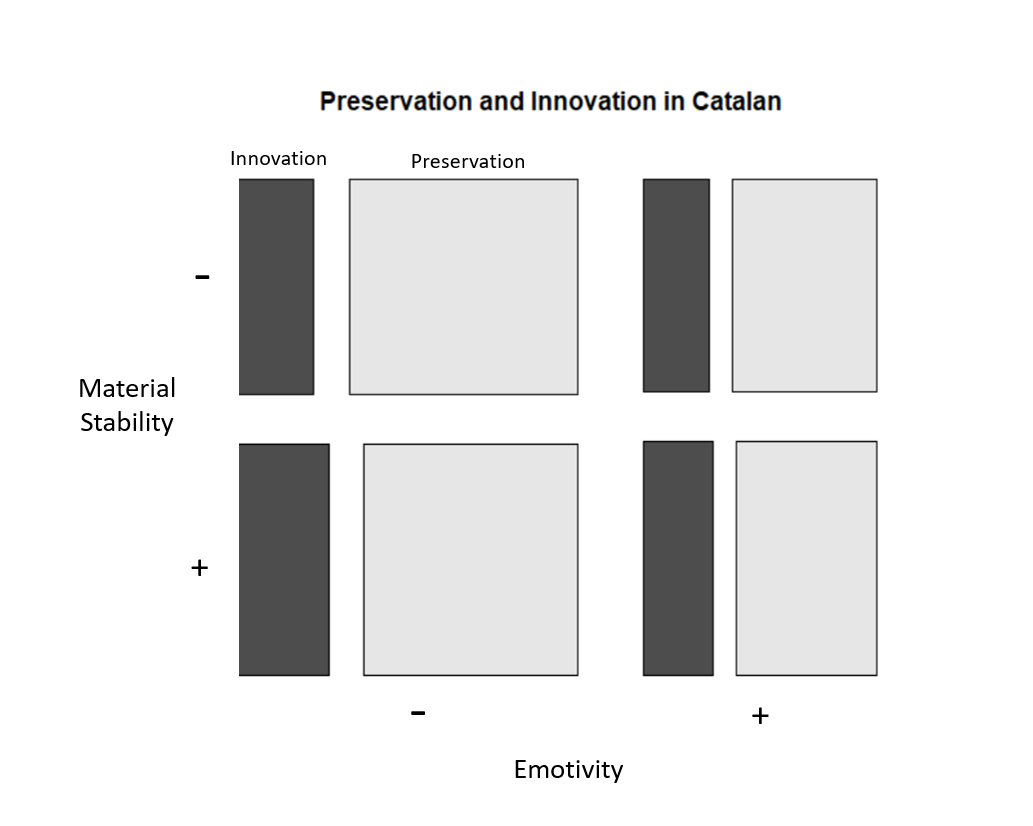
\includegraphics[width=.45\textwidth]{../figures/weiher_FINAL-cat}
%     \label{fig:weiher:cat}
% }
% \subfigure[Preservation and innovation in French]{
%     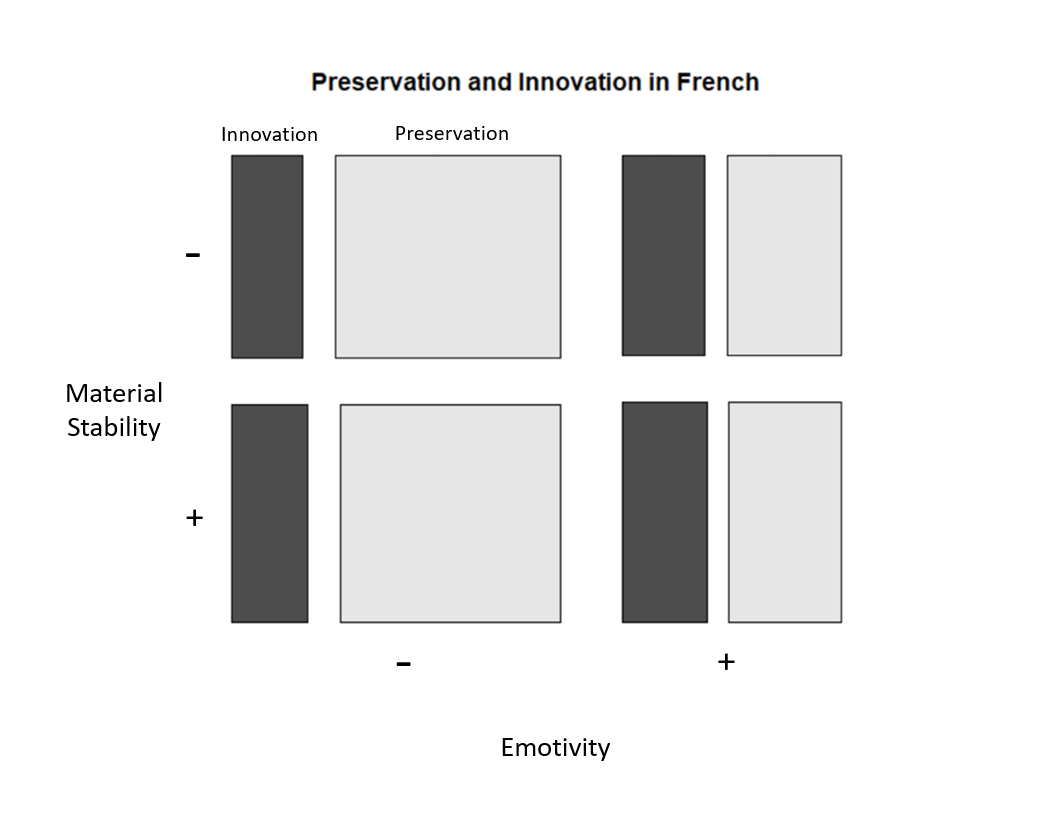
\includegraphics[width=.45\textwidth]{../figures/weiher_FINAL-fr}
%     \label{fig:weiher:fr}
% }\newline

% \subfigure[Preservation and innovation in Italian]{
%     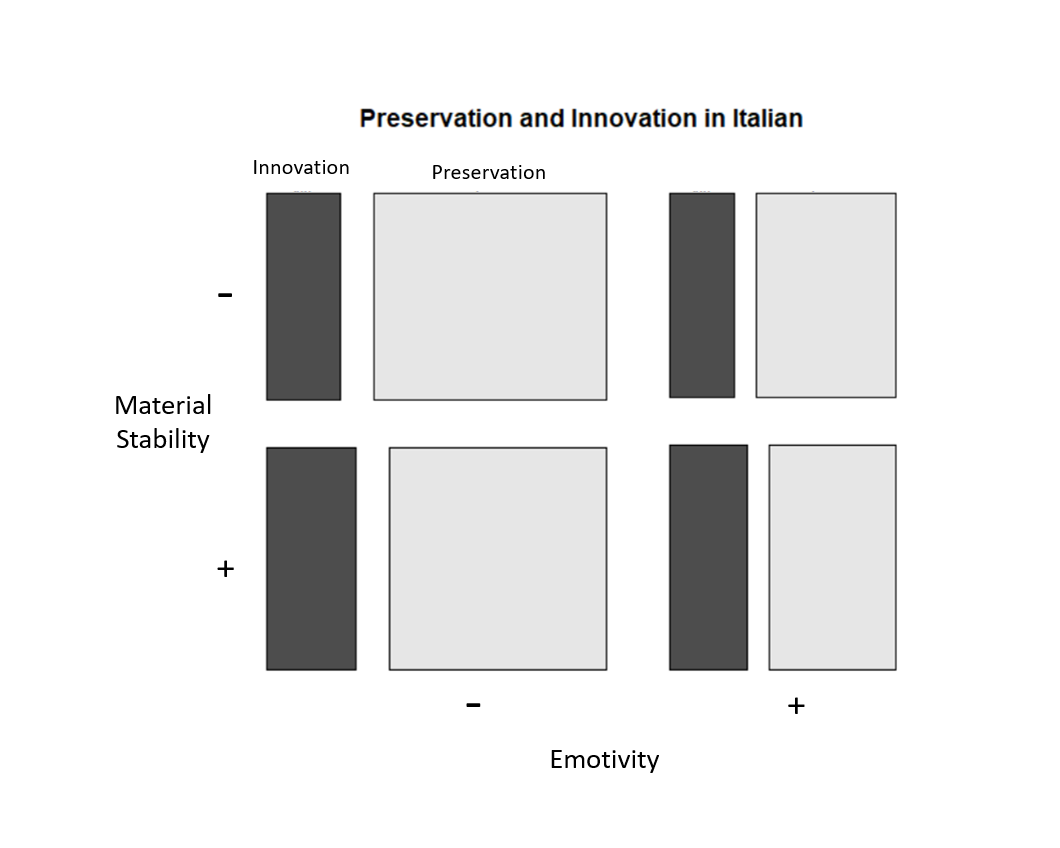
\includegraphics[width=.45\textwidth]{../figures/weiher_FINAL-ita}
%     \label{fig:weiher:ita}
% }
% \subfigure[Preservation and innovation in Portuguese]{
%     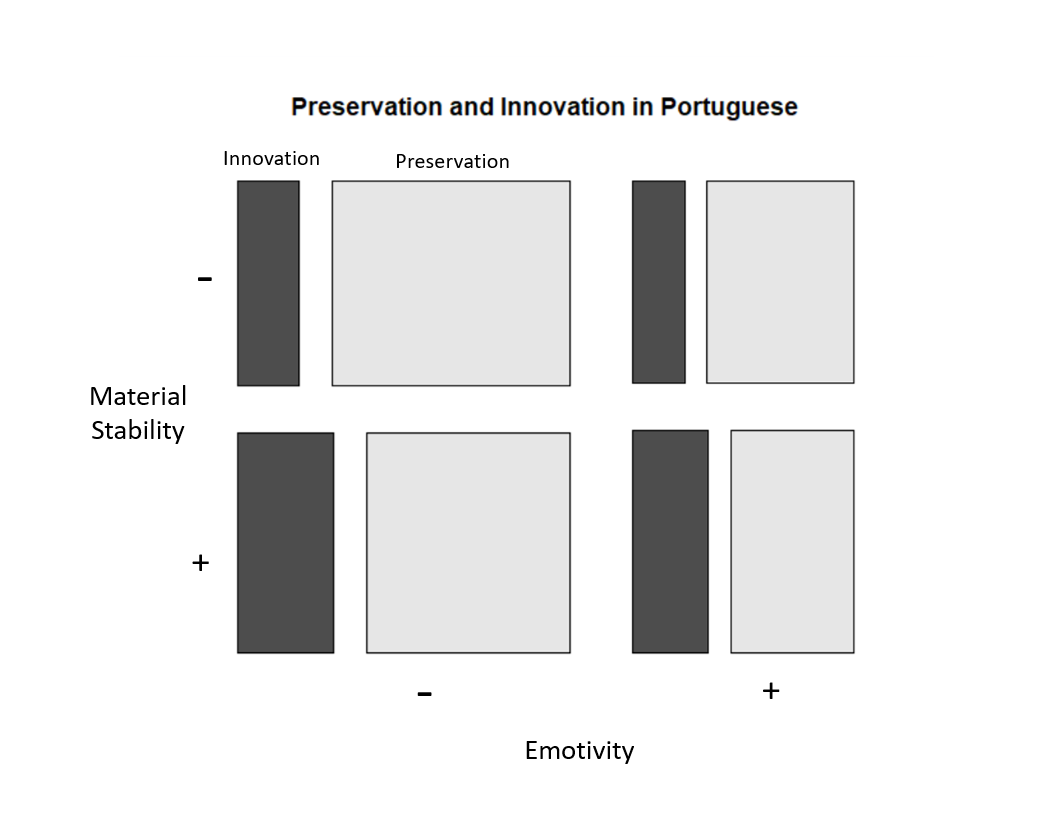
\includegraphics[width=.45\textwidth]{../figures/weiher_FINAL-po}
%     \label{fig:weiher:port}
% }\newline

% \subfigure[Preservation and innovation in Romanian]{
%     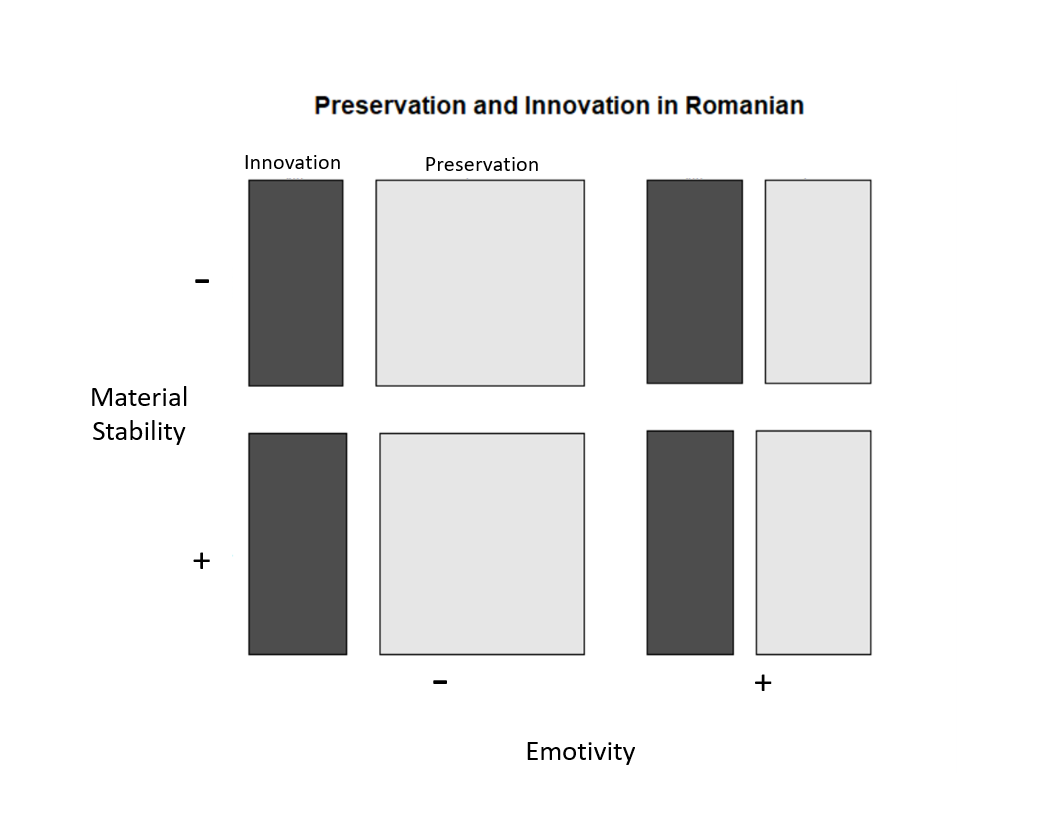
\includegraphics[width=.45\textwidth]{../figures/weiher_FINAL-ro.png}
%     \label{fig:weiher:ro}
% }
% \subfigure[Preservation and innovation in Spanish]{
%     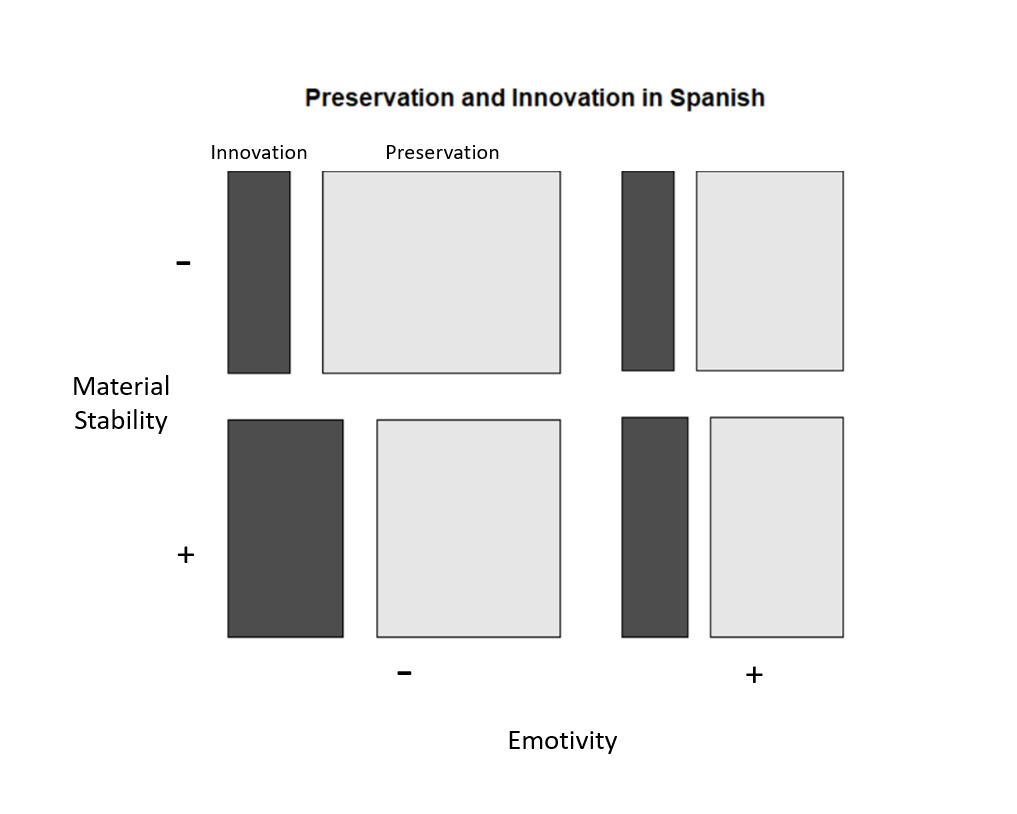
\includegraphics[width=.45\textwidth]{../figures/weiher_FINAL-spa.png}
%     \label{fig:weiher:spa}
% }
% \end{figure}

\todo[inline]{I noticed the preservation and innovation figures are not uniform (the boxes have different heights). Shall we redraw them as images or convert to a LaTeX-based plot?}
\begin{figure}[h]
    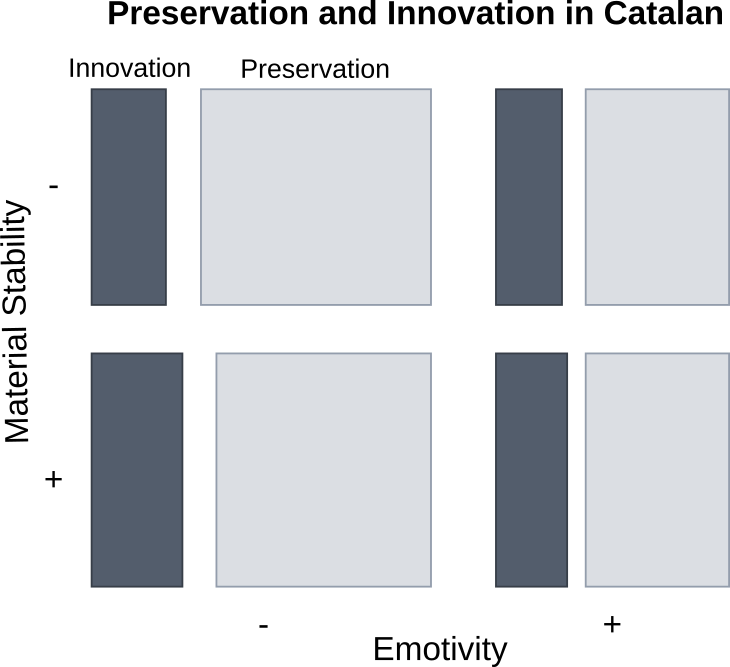
\includegraphics[width=\textwidth]{../figures/weiher_FINAL-cat1}
    \caption{Preservation and innovation in Catalan}
    \label{fig:weiher:cat}
\end{figure}

\begin{figure}[h]
    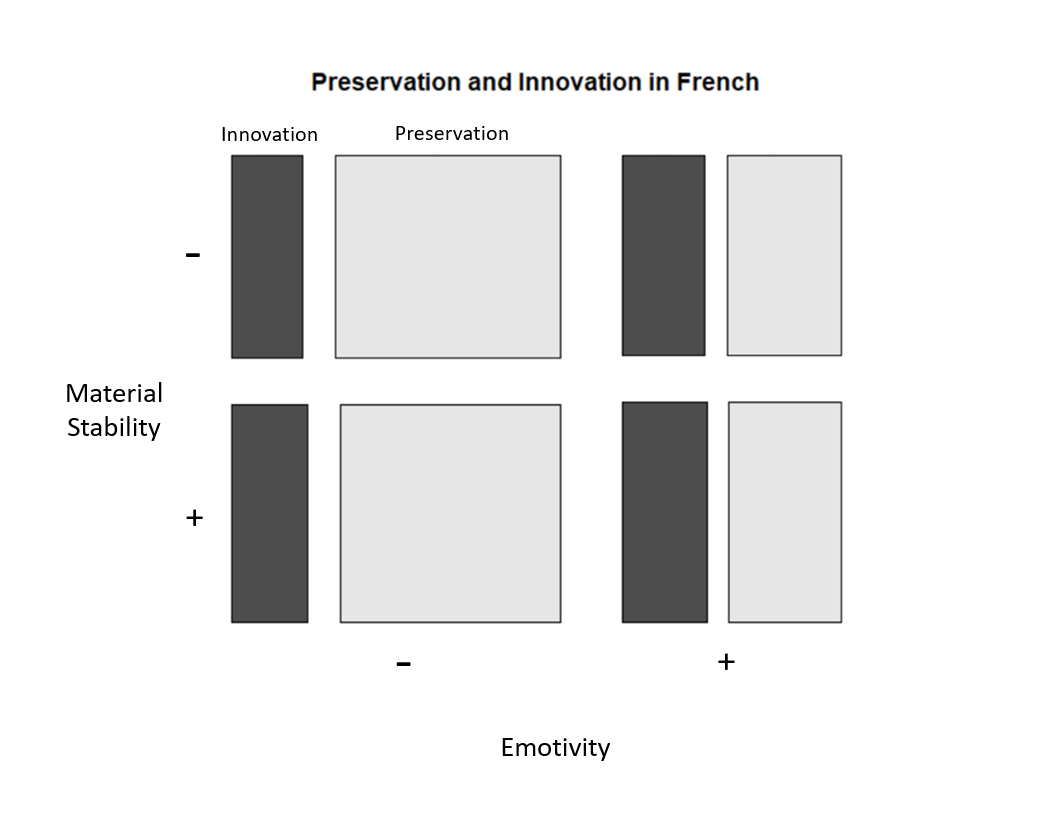
\includegraphics[width=\textwidth]{../figures/weiher_FINAL-fr}
    \caption{Preservation and innovation in French} 
    \label{fig:weiher:fr}
\end{figure}

\begin{figure}[h]
    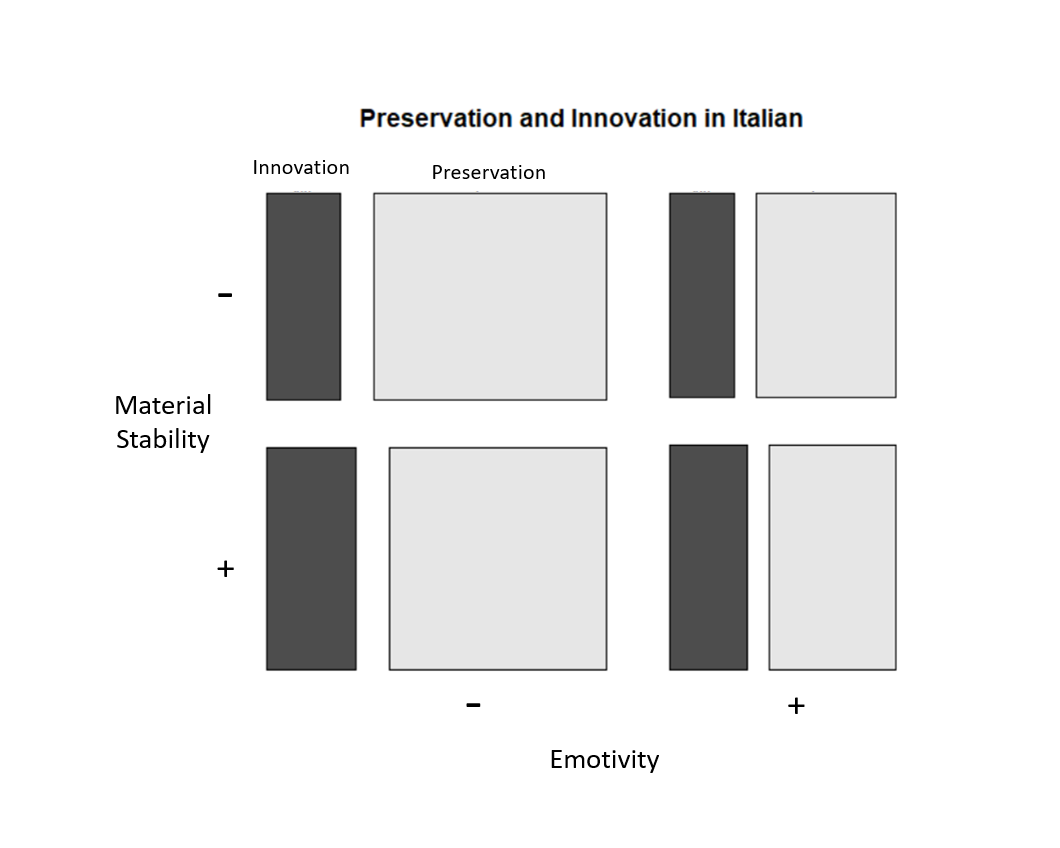
\includegraphics[width=\textwidth]{../figures/weiher_FINAL-ita}
    \caption{Preservation and innovation in Italian} 
    \label{fig:weiher:ita}
\end{figure}

\begin{figure}[h]
    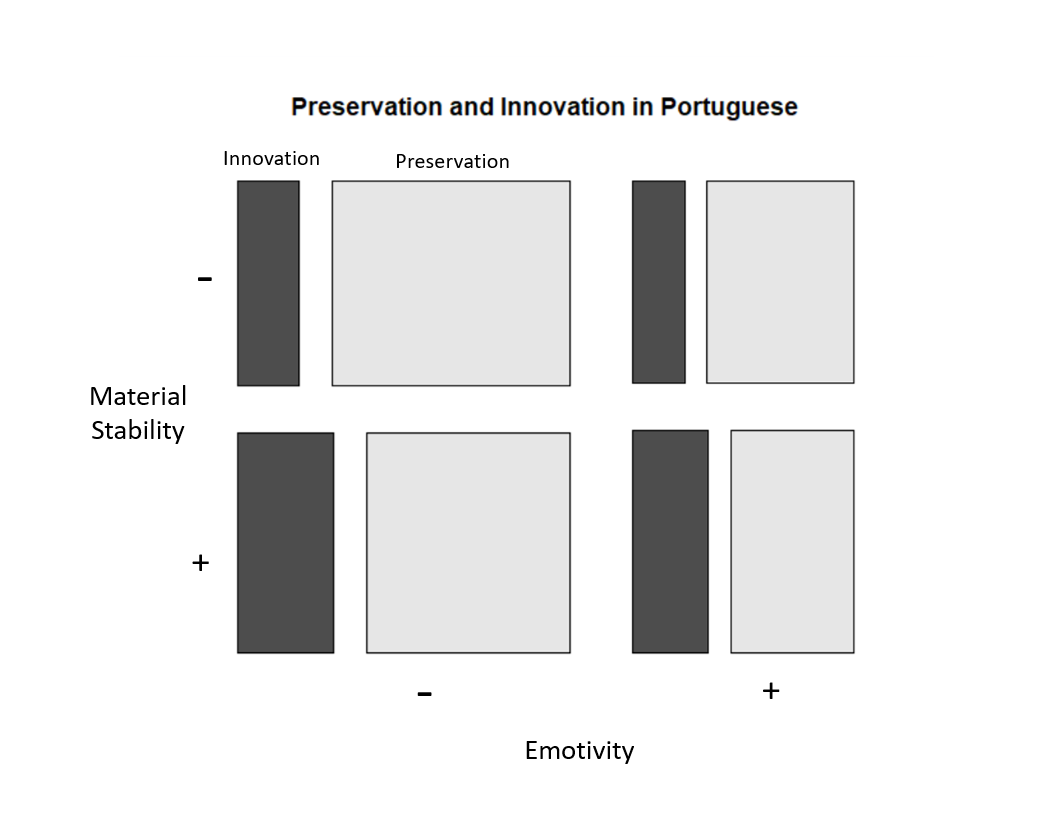
\includegraphics[width=\textwidth]{../figures/weiher_FINAL-po}
    \caption{Preservation and innovation in Portuguese} 
    \label{fig:weiher:port}
\end{figure}

\begin{figure}[h]
    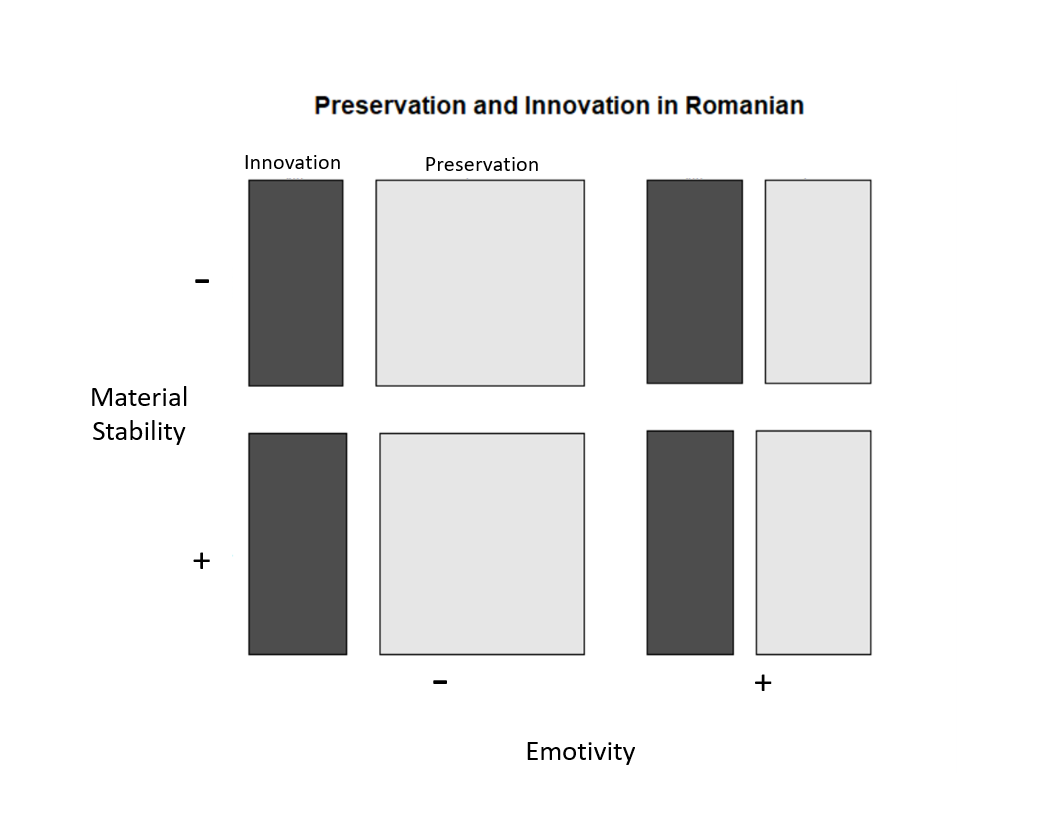
\includegraphics[width=\textwidth]{../figures/weiher_FINAL-ro.png}
    \caption{Preservation and innovation in Romanian} 
    \label{fig:weiher:ro}
\end{figure}

\begin{figure}[h]
    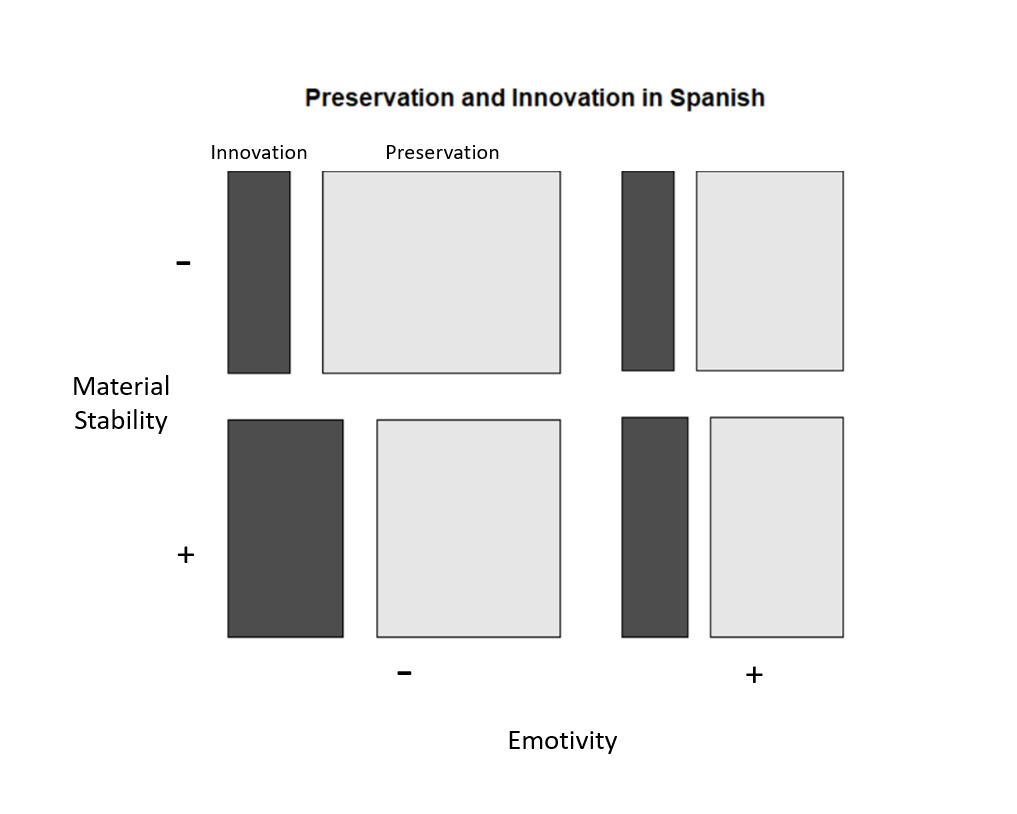
\includegraphics[width=\textwidth]{../figures/weiher_FINAL-spa.png}
    \caption{Preservation and innovation in Spanish} 
    \label{fig:weiher:spa}
\end{figure}
%I'm unsure how to get these to appear together rather than spaced out throughout several paragraphs. 

\subsection{Discussion}
When considering the Romance varieties in terms of their Latinate nature, \citet[326]{posner_romance_1996} remarks that, while some classify certain Romance varieties as more conservative than others, ‘conservative’ is rarely well-defined. For instance, conservatism could be determined by the presence or lack of nearly pan-Romance phonological changes (e.g. the case of Sardinian), or by the maintenance or loss of Latin culture, or even by geographic distance from “innovatory centers,” as in the case of Portuguese (326--327). Thus, in previous histories of Romance, there is a tendency to place languages in hierarchies according to the presence or absence of an arbitrary combination of linguistic changes.

Stefenelli’s (1992, as cited in \citealt{stefenelli_lexical_2011}) claims, however, are focused on the Latinate nature of the lexicon specifically. In his accounts of the lexical development of the Romance languages, he proposes a set of core factors that mediate lexical stability and innovation, two of which have been submitted to quantitative inquiry in the present study. First, material stability has previously been suggested to mediate lexical stability, and results of statistical analysis support this claim. Specifically, whereas lexical preservation occurred at a frequency of 65.7\% in our Romance sample for forms coded -Material Stability, this figure rose to 71.5\% for items coded +Material Stability. There is also a significant interaction between material stability and emotivity, such that emotivity nullifies the effect of material stability when the two factors operate together. This result corroborates another claim made in both \citealt[325]{posner_romance_1996} and in \citealt[580]{stefenelli_lexical_2011}, that the emotive value of a term disrupts the stabilizing effects of other factors. Conversely, though emotivity is confirmed by these data to have some kind of effect on lexical preservation, the results of the present experiment do not corroborate the notion that emotivity promotes preservation.

In addition to his claims about the factors at play in lexical stability, Stefenelli (1992, as cited in \citealt[569]{stefenelli_lexical_2011}) draws on counts of preservation of the “thousand most frequent central lexemes of (written) Latin” in a selection of nine Romance varieties to propose a hierarchy of stability, reproduced with the six-language sample of the present study in Figure 7. According to this hierarchy, Italian is the most Latinate and Romanian is the least (582).

\begin{figure}
    
    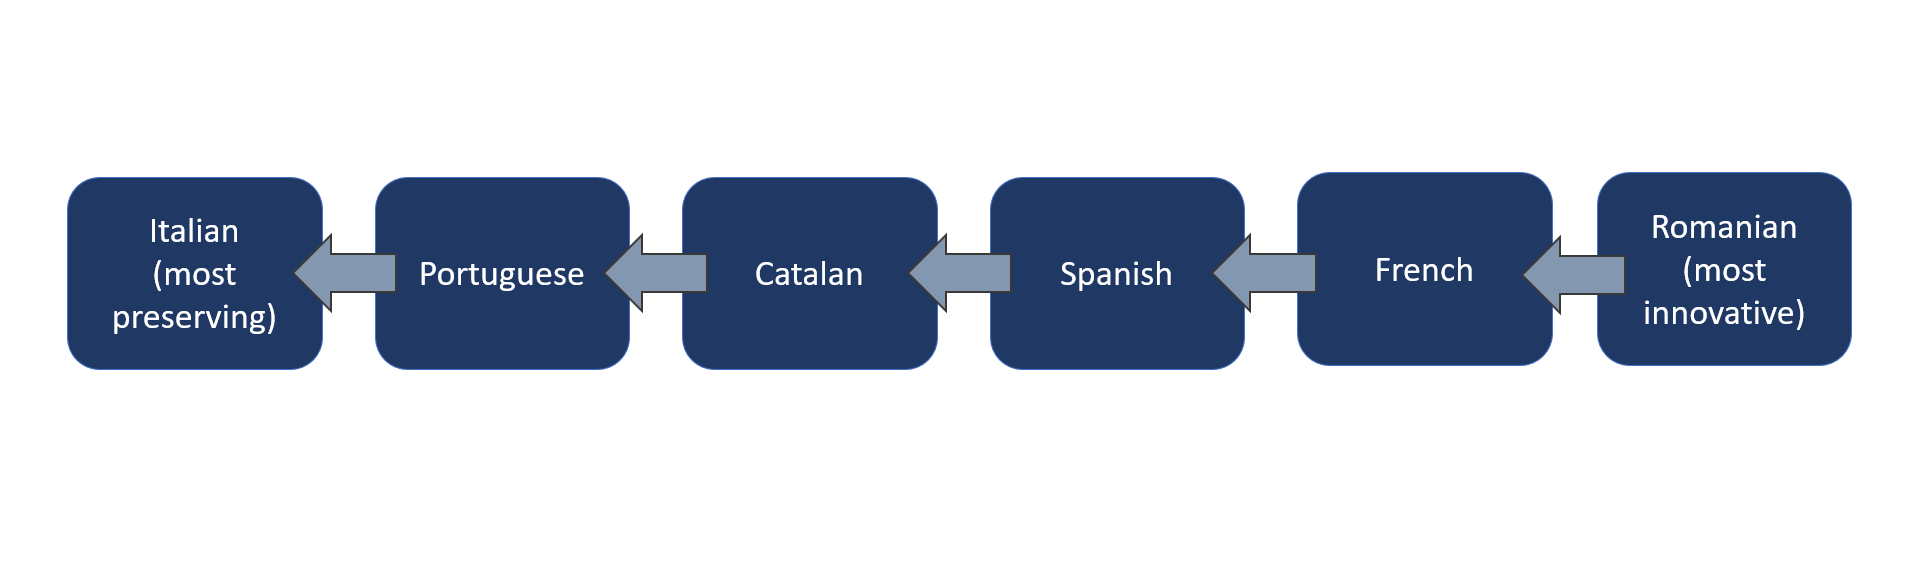
\includegraphics[width=\textwidth]{../figures/weiher_hierarchy}
    \caption{Hierarchy of preservation in \citet{stefenelli_lexical_2011}} 
    \label{fig:weiher:galaxy}
\end{figure}

This proposed hierarchy would suggest an effect of individual language on preservation. However, the results of the present study do not find sufficient evidence of this effect, as demonstrated by the lack of selection of Language as a main effect in the step-wise regression model. Nevertheless, it is important to note that the present experiment examines lexical stability at two points across a large time span, that is, from Classical Latin to the contemporary Romance lexicon. When contrasted with earlier stages of development of the Romance languages, \citet[583]{stefenelli_lexical_2011} observes a slightly different hierarchy, demonstrating how the Latinate nature of a given variety in relation to others differs across the span of its development. Moreover, Stefenelli clarifies that much like Latin, the early Romance varieties should be viewed as “diasystems,” each subject to considerable variation and not diachronically monolithic (\textit{ibid}). Of course, both Stefenelli’s analysis and the present experiment are focused strictly on lexical preservation as mediated by select factors, and there are other interpretations of the Latinate nature of the Romance languages based on stability in other linguistic domains, such as phonology (cf. \citealt[326--327]{posner_romance_1996}). Thus, we might view this claim as a part of the larger notion of a hierarchy of Latinity in Romance, which may differ by domain.

\section*{Conclusion}
In the transition from Latin to Romance, it is posited that lexical preservation is mediated by a series of linguistic factors, including material stability and emotivity (\citealt{posner_romance_1996}, \citealt{glessgen_linguistique_2007}, \citealt{stefenelli_lexical_2011}). The present study submits these more impressionistic claims to empirical investigation by examining the rates of preservation and innovation of a stratified random sampling of basic Latin vocabulary in six Romance varieties, as mediated by the factors material stability and emotivity.

Results of the present study lend evidence in support of Stefenelli’s (1992, as cited in \citealt{stefenelli_lexical_2011}) claims about the variables that mediate lexical preservation and innovation in Romance. Specifically, the claims that material stability promotes preservation, but that emotivity–when in interaction with material stability–disrupts preservation, are corroborated by these data. While these data do not corroborate Stefenelli’s proposed hierarchy of lexical stability, this does not eliminate the possibility such a hierarchy, or of parallel hierarchies of closeness to Latin in other domains. Thus, further empirical study of the Latinate nature of modern Romance is warranted, both at the level of the lexicon (with, perhaps, a larger data set and attention to the wider set of proposed factors) and in other domains. Once such tests are carried out in other areas of grammar (e.g. morphology, syntax, etc.), there may emerge a clearer ordering of Romance varieties by their closeness to Latin. Moreover, further study in this vein that treats a wider assortment of Romance varieties is needed in order to draw conclusions about Romance as a whole. This investigation, however, sheds some light on the nuances of previous observations (Stefenelli 1992, as cited in \citealt{stefenelli_lexical_2011}, \citealt{posner_romance_1996}, \citealt{glessgen_linguistique_2007}, \citealt{alkire_romance_2010}) about stability in the lexical development of Romance, and underscores the importance of marrying qualitative and quantitative research methodologies in the advancement of historical linguistic theory.

\section*{Acknowledgements}
I am first and foremost grateful to Justin Davidson for his assistance at several stages of the project, including the many rounds of feedback he provided on this manuscript. I am also grateful to my colleagues, Gabriella Licata, Ernesto Gutiérrez Topete and Ben Papadopolous, for their assistance with R and for their feedback during manuscript preparation. I am grateful to the two anonymous reviewers, whose suggestions were invaluable in revising this paper. Finally, I am grateful to the attendees of LSRL 49 for their thoughtful questions and contributions to the discussion of the project. 

\printbibliography[heading=subbibliography,notkeyword=this]
%NB: I've been unable to get the listing for the R Core Team to show as one 'name' rather than defaulting to Last, First format. 

\end{document}